% Options for packages loaded elsewhere
% Options for packages loaded elsewhere
\PassOptionsToPackage{unicode}{hyperref}
\PassOptionsToPackage{hyphens}{url}
\PassOptionsToPackage{dvipsnames,svgnames,x11names}{xcolor}
%
\documentclass[
  11pt,
  letterpaper,
]{article}
\usepackage{xcolor}
\usepackage[top=3cm,bottom=3cm,left=2.5cm,right=2.5cm]{geometry}
\usepackage{amsmath,amssymb}
\setcounter{secnumdepth}{-\maxdimen} % remove section numbering
\usepackage{iftex}
\ifPDFTeX
  \usepackage[T1]{fontenc}
  \usepackage[utf8]{inputenc}
  \usepackage{textcomp} % provide euro and other symbols
\else % if luatex or xetex
  \usepackage{unicode-math} % this also loads fontspec
  \defaultfontfeatures{Scale=MatchLowercase}
  \defaultfontfeatures[\rmfamily]{Ligatures=TeX,Scale=1}
\fi
\usepackage{lmodern}
\ifPDFTeX\else
  % xetex/luatex font selection
\fi
% Use upquote if available, for straight quotes in verbatim environments
\IfFileExists{upquote.sty}{\usepackage{upquote}}{}
\IfFileExists{microtype.sty}{% use microtype if available
  \usepackage[]{microtype}
  \UseMicrotypeSet[protrusion]{basicmath} % disable protrusion for tt fonts
}{}
\makeatletter
\@ifundefined{KOMAClassName}{% if non-KOMA class
  \IfFileExists{parskip.sty}{%
    \usepackage{parskip}
  }{% else
    \setlength{\parindent}{0pt}
    \setlength{\parskip}{6pt plus 2pt minus 1pt}}
}{% if KOMA class
  \KOMAoptions{parskip=half}}
\makeatother
% Make \paragraph and \subparagraph free-standing
\makeatletter
\ifx\paragraph\undefined\else
  \let\oldparagraph\paragraph
  \renewcommand{\paragraph}{
    \@ifstar
      \xxxParagraphStar
      \xxxParagraphNoStar
  }
  \newcommand{\xxxParagraphStar}[1]{\oldparagraph*{#1}\mbox{}}
  \newcommand{\xxxParagraphNoStar}[1]{\oldparagraph{#1}\mbox{}}
\fi
\ifx\subparagraph\undefined\else
  \let\oldsubparagraph\subparagraph
  \renewcommand{\subparagraph}{
    \@ifstar
      \xxxSubParagraphStar
      \xxxSubParagraphNoStar
  }
  \newcommand{\xxxSubParagraphStar}[1]{\oldsubparagraph*{#1}\mbox{}}
  \newcommand{\xxxSubParagraphNoStar}[1]{\oldsubparagraph{#1}\mbox{}}
\fi
\makeatother


\usepackage{longtable,booktabs,array}
\newcounter{none} % for unnumbered tables
\usepackage{calc} % for calculating minipage widths
% Correct order of tables after \paragraph or \subparagraph
\usepackage{etoolbox}
\makeatletter
\patchcmd\longtable{\par}{\if@noskipsec\mbox{}\fi\par}{}{}
\makeatother
% Allow footnotes in longtable head/foot
\IfFileExists{footnotehyper.sty}{\usepackage{footnotehyper}}{\usepackage{footnote}}
\makesavenoteenv{longtable}
\usepackage{graphicx}
\makeatletter
\newsavebox\pandoc@box
\newcommand*\pandocbounded[1]{% scales image to fit in text height/width
  \sbox\pandoc@box{#1}%
  \Gscale@div\@tempa{\textheight}{\dimexpr\ht\pandoc@box+\dp\pandoc@box\relax}%
  \Gscale@div\@tempb{\linewidth}{\wd\pandoc@box}%
  \ifdim\@tempb\p@<\@tempa\p@\let\@tempa\@tempb\fi% select the smaller of both
  \ifdim\@tempa\p@<\p@\scalebox{\@tempa}{\usebox\pandoc@box}%
  \else\usebox{\pandoc@box}%
  \fi%
}
% Set default figure placement to htbp
\def\fps@figure{htbp}
\makeatother





\setlength{\emergencystretch}{3em} % prevent overfull lines

\providecommand{\tightlist}{%
  \setlength{\itemsep}{0pt}\setlength{\parskip}{0pt}}



 
\usepackage[style=apa]{biblatex}
\addbibresource{referencias.bib}


% ==============================================================
% PAQUETES Y CONFIGURACIÓN BASE
% ==============================================================
\usepackage[utf8]{inputenc}
\usepackage[T1]{fontenc}
\usepackage[spanish, es-nodecimaldot]{babel}

% --- Fuente Palatino ---
\usepackage{mathpazo}
\linespread{1.05}
\usepackage{textcomp}

% --- Matemáticas ---
\usepackage{amsmath, amssymb, amsthm, mathtools, cancel}

% --- Diseño y Tablas ---
\usepackage{enumitem, booktabs, fancyhdr, titlesec, tabularx}
\usepackage{graphicx, float, subcaption}

% --- Cajas y Diagramas ---
\usepackage[most]{tcolorbox}
\usepackage{tikz, tikz-cd}

% --- Referencias cruzadas ---
\usepackage{hyperref}
\hypersetup{
    colorlinks  = true,
    linkcolor   = MidnightBlue,
    citecolor   = Teal,
    urlcolor    = DarkSlateGray
}
\usepackage[spanish]{cleveref}

% ==============================================================
% PALETA DE COLORES
% ==============================================================
\colorlet{colordef}{MidnightBlue}
\colorlet{colorteor}{Teal}
\colorlet{colorej}{DarkSlateGray}
\colorlet{colorobs}{DimGray}

% ==============================================================
% ESTILOS DE CAJAS (tcolorbox)
% ==============================================================
\tcbset{
    theorembase/.style={
        fonttitle            = \bfseries\sffamily\small,
        separator sign       = {\ ---},
        description delimiters = {(}{)},
        terminator sign      = {.},
        before upper         = {\parindent 1.5em},
        breakable,
        enhanced,
        attach boxed title to top left = {yshift = -2mm, xshift = 4mm},
        boxed title style    = {sharp corners, size = small},
        sharp corners,
        top = 4mm,
    },
    defstyle/.style={
        theorembase,
        colback      = colordef!4!white,
        colframe     = colordef!50!black,
        colbacktitle = colordef!70!black,
        coltitle     = white,
    },
    teorstyle/.style={
        theorembase,
        colback      = colorteor!4!white,
        colframe     = colorteor!55!black,
        colbacktitle = colorteor!75!black,
        coltitle     = white,
    },
    ejstyle/.style={
        theorembase,
        colback      = colorej!4!white,
        colframe     = colorej!45!black,
        colbacktitle = colorej!65!black,
        coltitle     = white,
    },
    obsstyle/.style={
        enhanced,
        breakable,
        fonttitle       = \bfseries\sffamily\small,
        separator sign  = {\ ---},
        description delimiters = {(}{)},
        terminator sign = {.},
        before upper    = {\parindent 1.5em},
        attach boxed title to top left = {yshift = -2mm, xshift = 4mm},
        boxed title style = {sharp corners, size = small,
                             colback = colorobs!60!black, coltitle = white},
        colback  = colorobs!4!white,
        colframe = colorobs!4!white,
        borderline west = {2.5pt}{0pt}{colorobs!70!black},
        top = 4mm,
    },
}

% ==============================================================
% AMBIENTES DE TEOREMAS
% ==============================================================
\newtcbtheorem[number within = section]{teorema}{Teorema}{teorstyle}{thm}
\newtcbtheorem[use counter from = teorema]{lema}{Lema}{teorstyle}{lem}
\newtcbtheorem[use counter from = teorema]{proposicion}{Proposición}{teorstyle}{prop}
\newtcbtheorem[use counter from = teorema]{corolario}{Corolario}{teorstyle}{cor}
\newtcbtheorem[number within = section]{definicion}{Definición}{defstyle}{def}
\newtcbtheorem[number within = section]{ejemplo}{Ejemplo}{ejstyle}{ej}
\newtcbtheorem[number within = section]{observacion}{Observación}{obsstyle}{obs}
\newtcbtheorem[number within = section]{ejercicio}{Ejercicio}{obsstyle}{exer}

\renewcommand{\proofname}{Demostración}

% ==============================================================
% MACROS MATEMÁTICAS
% ==============================================================
\newcommand{\N}{\ensuremath{\mathbb{N}}}
\newcommand{\Z}{\ensuremath{\mathbb{Z}}}
\newcommand{\Q}{\ensuremath{\mathbb{Q}}}
\newcommand{\R}{\ensuremath{\mathbb{R}}}
\newcommand{\C}{\ensuremath{\mathbb{C}}}

\newcommand{\eps}{\varepsilon}
\newcommand{\del}{\delta}

\DeclarePairedDelimiter{\abs}{\lvert}{\rvert}
\DeclarePairedDelimiter{\norm}{\lVert}{\rVert}
\DeclarePairedDelimiter{\inner}{\langle}{\rangle}
\DeclarePairedDelimiter{\ceil}{\lceil}{\rceil}
\DeclarePairedDelimiter{\floor}{\lfloor}{\rfloor}

\DeclareMathOperator{\sen}{sen}
\DeclareMathOperator{\tg}{tg}
\DeclareMathOperator{\Img}{Im}
\DeclareMathOperator{\Ker}{Ker}
\DeclareMathOperator{\rango}{rango}

% ==============================================================
% FORMATO DE SECCIONES (titlesec)
% ==============================================================
\titleformat{\section}
    {\large\bfseries\sffamily}
    {\thesection.}{0.6em}{}
    [\vspace{2pt}\rule{\linewidth}{0.4pt}\vspace{-4pt}]

\titleformat{\subsection}
    {\normalsize\bfseries\sffamily}
    {\thesubsection.}{0.5em}{}

\titleformat{\subsubsection}
    {\normalsize\itshape}
    {\thesubsubsection.}{0.5em}{}

\titlespacing{\section}{0pt}{14pt plus 2pt minus 1pt}{6pt}
\titlespacing{\subsection}{0pt}{10pt plus 1pt minus 1pt}{4pt}

% ==============================================================
% ENCABEZADO Y PIE DE PÁGINA
% ==============================================================
\pagestyle{fancy}
\fancyhf{}
\fancyhead[L]{\small\textsc{\curso}}
\fancyhead[C]{\small\itshape\titulo}
\fancyhead[R]{\small\thepage}
\renewcommand{\headrulewidth}{0.4pt}
\renewcommand{\footrulewidth}{0pt}

\fancypagestyle{plain}{%
    \fancyhf{}
    \fancyfoot[C]{\small\thepage}
    \renewcommand{\headrulewidth}{0pt}
}

\setlength{\parskip}{6pt}
\setlength{\parindent}{1.5em}
\usepackage[T1]{fontenc}
\usepackage[utf8]{inputenc}
\usepackage{graphicx}
\usepackage{adjustbox}
\let\oldtabular\tabular
\let\endoldtabular\endtabular
\renewenvironment{tabular}{\begin{adjustbox}{max width=\textwidth}\oldtabular}{\endoldtabular\endadjustbox}
\newcommand{\titulo}{Etapa 2}
\newcommand{\subtitulo}{subtitulo}
\newcommand{\autor}{Angel Ruben Galindo Alvarez}
\newcommand{\matricula}{A00228356}
\newcommand{\curso}{MA2003B Análisis Multivariado}
\newcommand{\profesor}{Blanca Rosa Ruiz Hernández \\ Raúl Gómez Muñoz}
\newcommand{\campus}{Campus Monterrey}
\newcommand{\fecha}{\today}
\makeatletter
\@ifpackageloaded{caption}{}{\usepackage{caption}}
\AtBeginDocument{%
\ifdefined\contentsname
  \renewcommand*\contentsname{Table of contents}
\else
  \newcommand\contentsname{Table of contents}
\fi
\ifdefined\listfigurename
  \renewcommand*\listfigurename{List of Figures}
\else
  \newcommand\listfigurename{List of Figures}
\fi
\ifdefined\listtablename
  \renewcommand*\listtablename{List of Tables}
\else
  \newcommand\listtablename{List of Tables}
\fi
\ifdefined\figurename
  \renewcommand*\figurename{Figure}
\else
  \newcommand\figurename{Figure}
\fi
\ifdefined\tablename
  \renewcommand*\tablename{Table}
\else
  \newcommand\tablename{Table}
\fi
}
\@ifpackageloaded{float}{}{\usepackage{float}}
\floatstyle{ruled}
\@ifundefined{c@chapter}{\newfloat{codelisting}{h}{lop}}{\newfloat{codelisting}{h}{lop}[chapter]}
\floatname{codelisting}{Listing}
\newcommand*\listoflistings{\listof{codelisting}{List of Listings}}
\makeatother
\makeatletter
\makeatother
\makeatletter
\@ifpackageloaded{caption}{}{\usepackage{caption}}
\@ifpackageloaded{subcaption}{}{\usepackage{subcaption}}
\makeatother
\usepackage{bookmark}
\IfFileExists{xurl.sty}{\usepackage{xurl}}{} % add URL line breaks if available
\urlstyle{same}
% fallback for those not using the hyperref driver hyperxmp:
\makeatletter
\@ifundefined{xmpquote}{\newcommand{\xmpquote}[1]{#1}}{}
\makeatother
\hypersetup{
  pdftitle={Comprensión de los datos y descripción de variables},
  colorlinks=true,
  linkcolor={blue},
  filecolor={Maroon},
  citecolor={Blue},
  urlcolor={Blue},
  pdfcreator={LaTeX via pandoc}}


\title{Comprensión de los datos y descripción de variables}
\author{}
\date{}
\begin{document}
\maketitle

\begin{titlepage}
\centering
\thispagestyle{empty}

{\small\textsc{Instituto Tecnológico y de Estudios Superiores de Monterrey}}

\vspace{0.6cm}

\includegraphics[scale=0.15]{logo.png}

\vspace{0.8cm}
{\color{colordef!70!black}\rule{\linewidth}{1pt}}
\vspace{0.8cm}

{\LARGE\bfseries \titulo}

\vspace{0.4cm}

{\large\itshape \subtitulo}

\vspace{1cm}

{\normalsize\textsc{\autor\ $\cdot$\ \matricula}}

\vspace{0.6cm}

{\small \curso\quad\textbar\quad\profesor}

\vfill

{\color{colordef!70!black}\rule{\linewidth}{0.6pt}}

\vspace{0.4cm}

\noindent{\small\textsc{\campus}\hfill\textsc{\fecha}}

\end{titlepage}

\tableofcontents
\newpage


\section{Objetivo del análisis y justificación del
alcance}\label{objetivo-del-anuxe1lisis-y-justificaciuxf3n-del-alcance}

\subsubsection{Pregunta de
investigación:}\label{pregunta-de-investigaciuxf3n}

¿De qué manera influyen las variables del clima en los picos de
contaminación (\(PM_{10}\), \(PM_{2.5}\) y \(O_{3}\)) dentro de las
distintas estaciones de monitoreo del Área Metropolitana de Monterrey
entre 2020 y 2025?

\subsubsection{Objetivo general:}\label{objetivo-general}

Crear y validar modelos predictivos utilizando datos históricos de 2020
a 2025 para estimar las concentraciones de PM10, PM2.5 y O3 en conjunto.
La idea es identificar qué factores climáticos detonan las contingencias
en cada zona y darle al SIMA una herramienta práctica para poder
anticiparlas.

Decidimos mantener el análisis de los contaminantes integrado porque,
aunque las partículas (\(PM_{10}\) y \(PM_{2.5}\)) comparten fuentes de
emisión y se comportan de forma muy similar, el ozono (\(O_{3}\))
funciona diferente al depender mucho más del calor y la radiación solar.
Juntar ambos comportamientos en un solo sistema resulta mucho más útil
para tomar decisiones públicas que si hiciéramos modelos separados.

\section{Técnicas estadísticas}\label{tuxe9cnicas-estaduxedsticas}

Para cumplir con este objetivo y asegurarnos de que el SIMA pueda
interpretar los resultados fácilmente para convertirlos en acciones,
utilizaremos las siguientes herramientas:

\begin{itemize}
\item
  Estadística descriptiva y detección de valores atípicos: Usaremos
  diagramas de caja para entender cuáles son los niveles ``normales'' de
  contaminación y aislar los días que realmente representan una
  contingencia en cada estación.
\item
  Análisis de correlación: Nos ayudará a ver cómo se relacionan los
  contaminantes entre sí (por ejemplo, la fuerte conexión entre PM10 y
  PM2.5) y cómo reaccionan a los cambios del clima, trabajando siempre
  con los datos en sus unidades originales.
\item
  Random Forest (Árboles de decisión): Elegimos este algoritmo porque
  hace pronósticos basados en reglas lógicas. Limitaremos qué tan
  complejos se vuelven estos árboles para que no se conviertan en una
  ``caja negra'' y siempre podamos explicar de dónde salió la
  predicción.
\end{itemize}

Para poder predecir la contaminación, trabajaremos con el archivo
SIMA\_Diario\_Imputado.csv, el cual consolida las lecturas por día.

Este archivo lo armamos uniendo seis documentos de Excel que contenían
el historial por hora (2020-2025) de las 15 estaciones de monitoreo de
Monterrey. Para hacer la información más manejable, sacamos los
promedios diarios, pero le pusimos una regla estricta: solo validamos
los días que tuvieran al menos 18 horas de mediciones reales. Los huecos
de información que quedaron por cualquier motivo los rellenamos
respetando el orden cronológico exacto de los días. Así nos aseguramos
de tener una base continua sin hacer ``trampa'' (mezclando información
del futuro en el pasado) antes de empezar a modelar. Cabe recalcar que
tambien respetamos el comportamiento de cada estación, es decir, no
imputamos los datos de una estacion el comportamiento de otra.

\subsubsection{Por qué es clave la estación de
monitoreo}\label{por-quuxe9-es-clave-la-estaciuxf3n-de-monitoreo}

La variable de la estación es una de las piezas más importantes del
proyecto. Como Monterrey está rodeado de montañas, se generan distintos
microclimas y ``trampas'' donde el aire se estanca. Esto significa que
la contaminación por PM10 en la zona suroeste no se comporta para nada
igual que en la zona sur. Si ignoramos de qué estación viene cada dato,
terminaríamos revolviendo todo y el modelo no entendería cómo se mueve y
dispersa realmente la contaminación en la ciudad.

\subsubsection{Diccionario de Variables}\label{diccionario-de-variables}

{\def\LTcaptype{none} % do not increment counter
\begin{longtable}[]{@{}
  >{\raggedright\arraybackslash}p{(\linewidth - 8\tabcolsep) * \real{0.2000}}
  >{\raggedright\arraybackslash}p{(\linewidth - 8\tabcolsep) * \real{0.2000}}
  >{\raggedright\arraybackslash}p{(\linewidth - 8\tabcolsep) * \real{0.2000}}
  >{\raggedright\arraybackslash}p{(\linewidth - 8\tabcolsep) * \real{0.2000}}
  >{\raggedright\arraybackslash}p{(\linewidth - 8\tabcolsep) * \real{0.2000}}@{}}
\toprule\noalign{}
\begin{minipage}[b]{\linewidth}\raggedright
Variable
\end{minipage} & \begin{minipage}[b]{\linewidth}\raggedright
Descripción
\end{minipage} & \begin{minipage}[b]{\linewidth}\raggedright
Tipo de Dato
\end{minipage} & \begin{minipage}[b]{\linewidth}\raggedright
Rango / Valores Posibles
\end{minipage} & \begin{minipage}[b]{\linewidth}\raggedright
Valores Nulos
\end{minipage} \\
\midrule\noalign{}
\endhead
\bottomrule\noalign{}
\endlastfoot
\textbf{Fecha} & Fecha cronológica de la lectura & Cualitativa (Ordinal)
& 2020-01-01 a 2025-12-31 & 0 \\
\textbf{Estacion} & Código de la estación de monitoreo & Cualitativa
(Nominal) & 15 valores (ej. CE, NE, SO, SUR) & 0 \\
\textbf{PM10} & Partículas menores a 10 micrómetros (Objetivo) &
Cuantitativa (Continua) & \(0 - >500 \, \mu\text{g/m}^3\) & 0 \\
\textbf{PM2.5} & Partículas menores a 2.5 micrómetros & Cuantitativa
(Continua) & \(0 - >300 \, \mu\text{g/m}^3\) & 0 \\
\textbf{TOUT} & Temperatura ambiente externa & Cuantitativa (Continua) &
\(-5.0 \text{ a } 45.0 \, ^\circ\text{C}\) & 0 \\
\textbf{RH} & Humedad relativa & Cuantitativa (Continua) &
\(0 \text{ a } 100\%\) & 0 \\
\textbf{WSR} & Velocidad del viento & Cuantitativa (Continua) &
\(0 \text{ a } 50 \text{ km/h}\) & 0 \\
\textbf{PRS} & Presión atmosférica & Cuantitativa (Continua) &
\(600 \text{ a } 800 \text{ mmHg}\) & 0 \\
\textbf{O3} & Ozono & Cuantitativa (Continua) &
\(0 \text{ a } 200 \text{ ppb}\) & 0 \\
\textbf{NO2} & Dióxido de nitrógeno & Cuantitativa (Continua) &
\(0 \text{ a } 100 \text{ ppb}\) & 0 \\
\textbf{CO} & Monóxido de carbono & Cuantitativa (Continua) &
\(0 \text{ a } 10 \text{ ppm}\) & 0 \\
\end{longtable}
}

\subsubsection{Características
Estadísticas}\label{caracteruxedsticas-estaduxedsticas}

\protect\phantomsection\label{exploracion-estadistica}
\protect\phantomsection\label{exploracion-estadistica-1}
\textbf{Dimensión del dataset:} 31449 registros y 18 columnas.

\protect\phantomsection\label{exploracion-estadistica-2}
\textbf{Estadísticas de Variables Cuantitativas:}

\protect\phantomsection\label{exploracion-estadistica-3}
{\def\LTcaptype{none} % do not increment counter
\begin{longtable}[]{@{}lllllll@{}}
\toprule\noalign{}
& mean & mediana & std & varianza & min & max \\
\midrule\noalign{}
\endhead
\bottomrule\noalign{}
\endlastfoot
Fecha & 2023-01-30 04:59:27.375751 & 2023-02-17 00:00:00 & NaN & NaN &
2020-01-01 00:00:00 & 2025-12-31 00:00:00 \\
Horas\_Registradas & 23.994499 & 24.0 & 0.081727 & 0.01 & 22.0 & 24.0 \\
CO & 1.320355 & 1.148413 & 0.853062 & 0.73 & 0.050417 & 9.206087 \\
NO & 15.319099 & 7.104348 & 29.273828 & 856.96 & 0.5 & 427.291667 \\
NO2 & 14.675147 & 12.725 & 8.882273 & 78.89 & 0.063158 & 95.179167 \\
NOX & 29.445311 & 20.28 & 32.504226 & 1056.52 & 0.5 & 457.954167 \\
O3 & 26.780897 & 26.5 & 9.423145 & 88.80 & 1.5 & 77.75 \\
PM10 & 57.462583 & 52.291667 & 27.849965 & 775.62 & 5.761905 &
301.541667 \\
PM2.5 & 20.266959 & 18.968571 & 10.175263 & 103.54 & 2.0 & 191.391304 \\
PRS & 715.236321 & 714.2625 & 9.26524 & 85.84 & 681.805556 &
747.666667 \\
RH & 55.001608 & 57.25 & 17.478992 & 305.52 & 1.47619 & 99.722222 \\
SO2 & 4.95991 & 4.145833 & 3.13212 & 9.81 & 0.585714 & 61.775 \\
SR & 0.147738 & 0.149083 & 0.234704 & 0.06 & 0.0 & 25.343208 \\
TOUT & 22.792355 & 24.51375 & 8.014495 & 64.23 & -57.794348 &
36.783889 \\
WDR & 140.977674 & 134.208333 & 62.15396 & 3863.11 & 1.454545 &
357.142857 \\
WSR & 8.31386 & 7.904167 & 4.734752 & 22.42 & 0.104348 & 158.858333 \\
RAINF & 0.71115 & 0.0 & 32.08521 & 1029.46 & 0.0 & 4897.1 \\
\end{longtable}
}

\protect\phantomsection\label{exploracion-estadistica-4}
\textbf{Tabla de Frecuencia (Variable Cualitativa - Estación):}

\protect\phantomsection\label{exploracion-estadistica-5}
{\def\LTcaptype{none} % do not increment counter
\begin{longtable}[]{@{}lll@{}}
\toprule\noalign{}
& Estacion & Frecuencia \\
\midrule\noalign{}
\endhead
\bottomrule\noalign{}
\endlastfoot
0 & CE & 2192 \\
1 & NE & 2192 \\
2 & NE2 & 2192 \\
3 & NO & 2192 \\
4 & NO2 & 2192 \\
5 & NTE & 2192 \\
6 & NTE2 & 2192 \\
7 & SE & 2192 \\
8 & SE2 & 2192 \\
9 & SE3 & 2192 \\
10 & SO & 2192 \\
11 & SO2 & 2192 \\
12 & SUR & 2192 \\
13 & NE3 & 1826 \\
14 & NO3 & 1127 \\
\end{longtable}
}

\section{Exploración Visual de los
Datos}\label{exploraciuxf3n-visual-de-los-datos}

A continuación, visualizamos el comportamiento de las variables
cuantitativas (distribución, asimetría, dispersión y correlación
multivariada) y cualitativas, utilizando la base de datos validada.

\pandocbounded{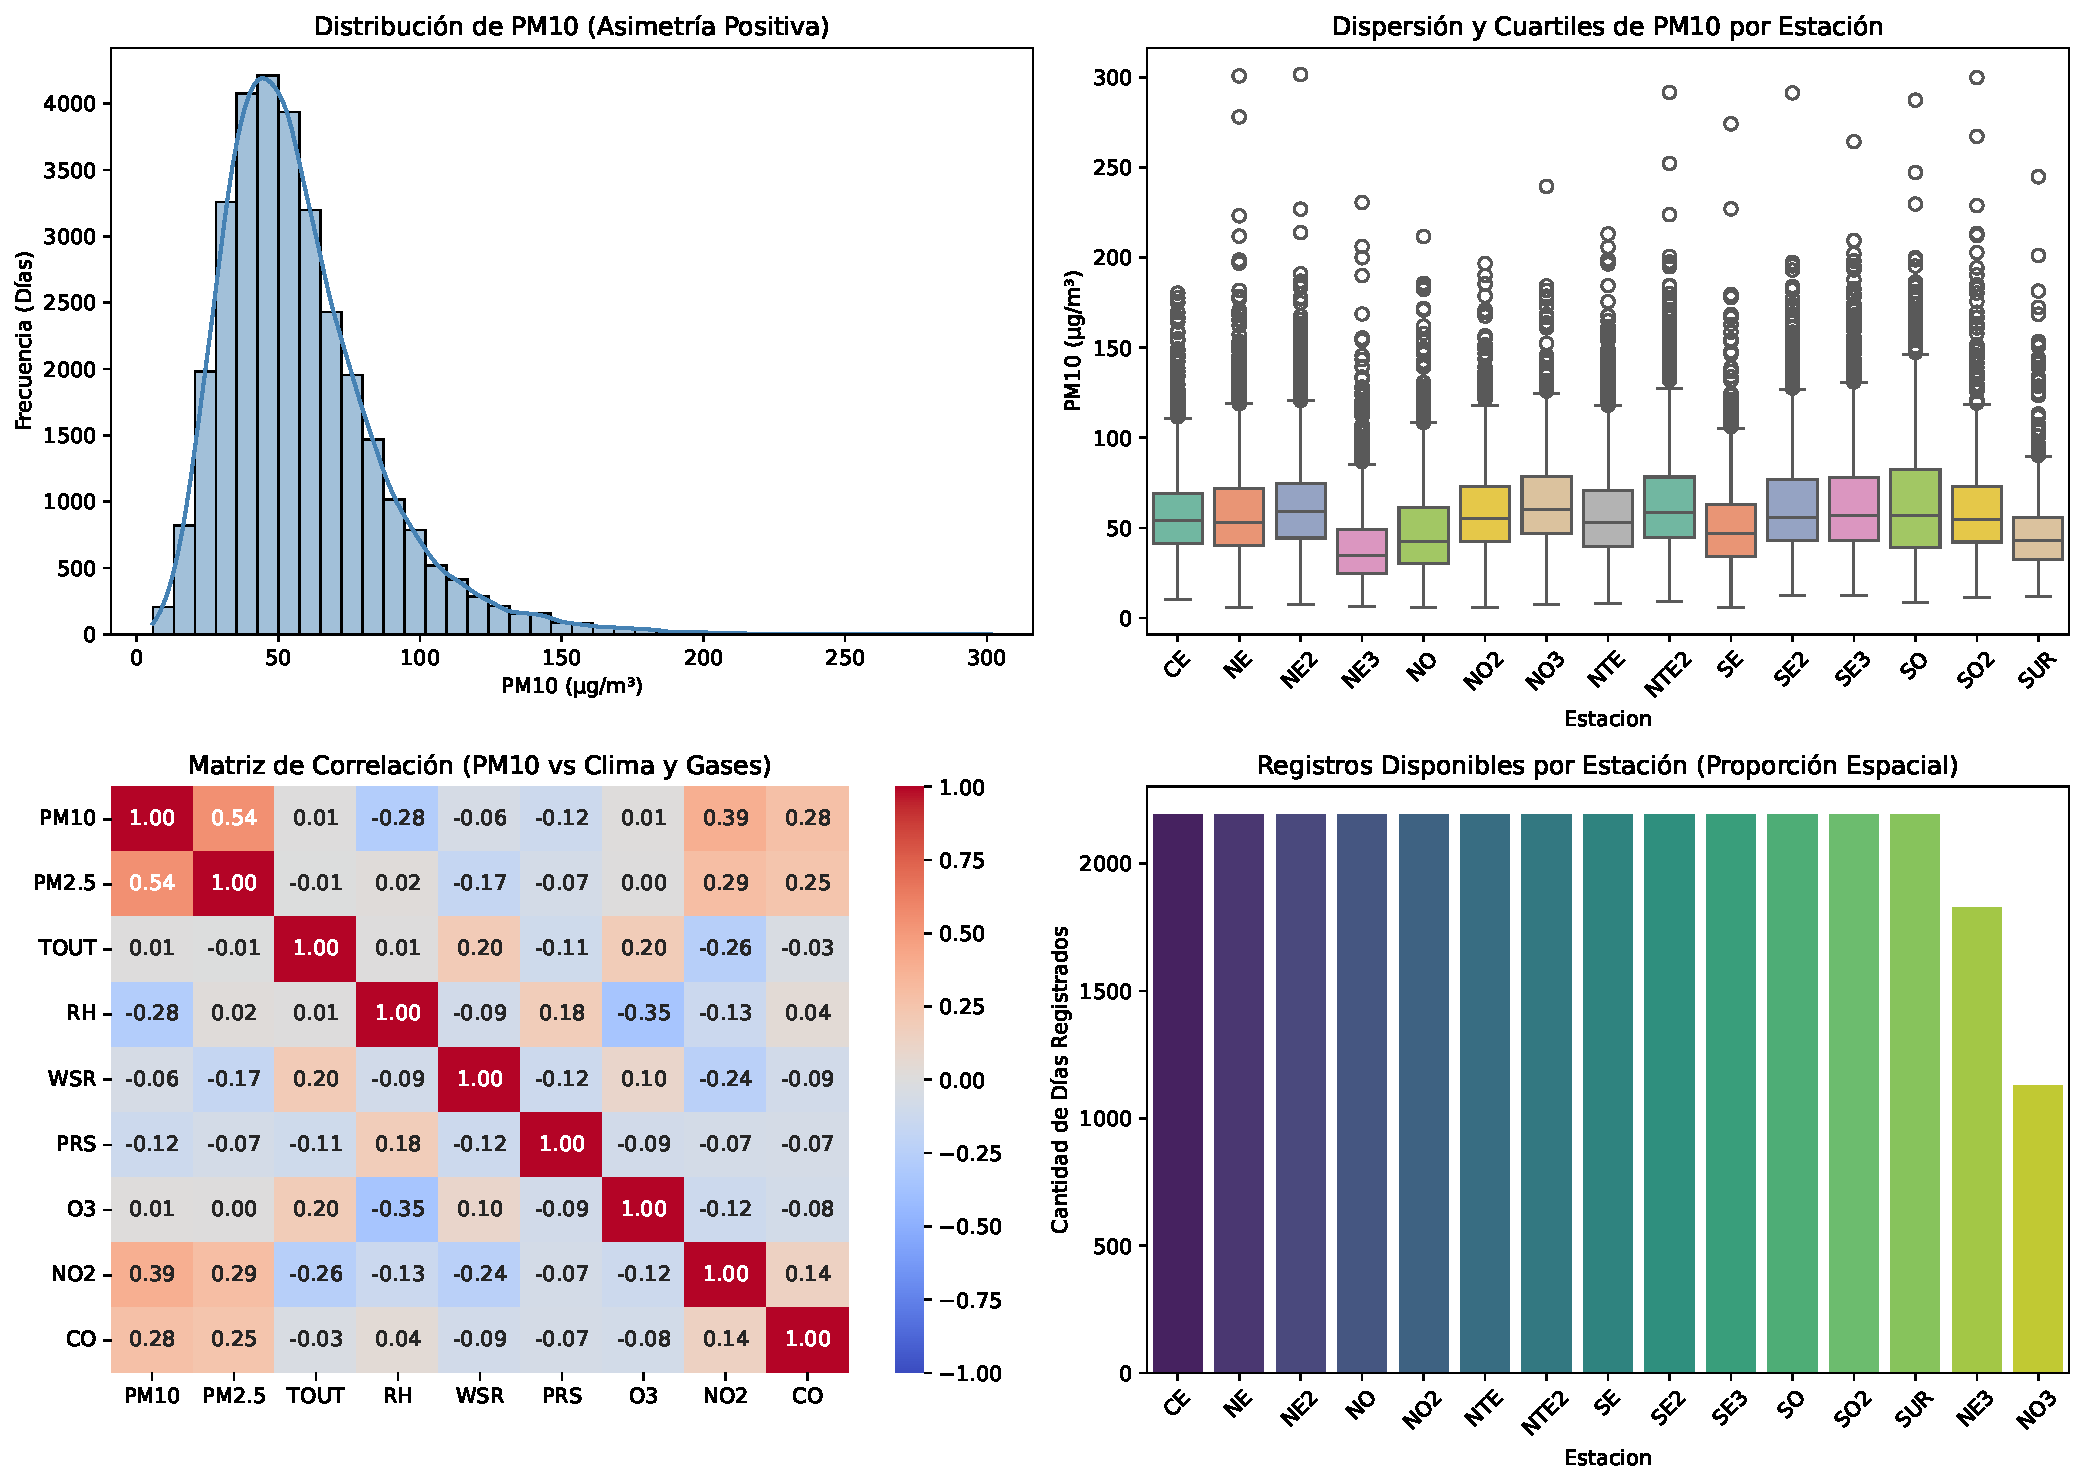
\includegraphics[keepaspectratio]{documento_files/figure-pdf/visualizacion-datos-output-1.pdf}}

\section{Verificación de la Calidad de los
Datos}\label{verificaciuxf3n-de-la-calidad-de-los-datos}

\protect\phantomsection\label{calidad-datos}
\protect\phantomsection\label{calidad-datos-1}
\begin{itemize}
\tightlist
\item
  \textbf{Valores Nulos:} 0 detectados.
\end{itemize}

\protect\phantomsection\label{calidad-datos-2}
\begin{itemize}
\tightlist
\item
  \textbf{Registros Duplicados:} 0 detectados.
\end{itemize}

\protect\phantomsection\label{calidad-datos-3}
\begin{itemize}
\tightlist
\item
  \textbf{Valores Negativos Inconsistentes:} 0 detectados.
\end{itemize}

\protect\phantomsection\label{calidad-datos-4}
\begin{itemize}
\tightlist
\item
  \textbf{Formato de Fechas Correcto:} Sí
\end{itemize}

\protect\phantomsection\label{calidad-datos-5}
\textbf{Conclusión de Calidad:} El dataset cumple con los criterios de
integridad necesarios para la siguiente fase de la metodología CRISP-DM.

\section{Selección de variables}\label{selecciuxf3n-de-variables}

En esta etapa, nos centramos en seleccionar las variables que nos
resulten más útiles para predecir la contaminación. Para ello,
utilizaremos algunas técnicas estadísticas para evaluar la calidad de
las variables y determinar cuáles son las más importantes para el
modelo.

\subsubsection{ANOVA}\label{anova}

Primero utilizaremos la técnica de ANOVA (Analysis of Variance).

{\def\LTcaptype{none} % do not increment counter
\begin{longtable}[]{@{}
  >{\raggedright\arraybackslash}p{(\linewidth - 12\tabcolsep) * \real{0.1429}}
  >{\raggedright\arraybackslash}p{(\linewidth - 12\tabcolsep) * \real{0.1429}}
  >{\raggedright\arraybackslash}p{(\linewidth - 12\tabcolsep) * \real{0.1429}}
  >{\raggedright\arraybackslash}p{(\linewidth - 12\tabcolsep) * \real{0.1429}}
  >{\raggedright\arraybackslash}p{(\linewidth - 12\tabcolsep) * \real{0.1429}}
  >{\raggedright\arraybackslash}p{(\linewidth - 12\tabcolsep) * \real{0.1429}}
  >{\raggedright\arraybackslash}p{(\linewidth - 12\tabcolsep) * \real{0.1429}}@{}}
\toprule\noalign{}
\begin{minipage}[b]{\linewidth}\raggedright
\end{minipage} & \begin{minipage}[b]{\linewidth}\raggedright
Variable
\end{minipage} & \begin{minipage}[b]{\linewidth}\raggedright
Levene\_p\_value
\end{minipage} & \begin{minipage}[b]{\linewidth}\raggedright
Homoscedastic
\end{minipage} & \begin{minipage}[b]{\linewidth}\raggedright
Test\_Used
\end{minipage} & \begin{minipage}[b]{\linewidth}\raggedright
ANOVA\_p\_value
\end{minipage} & \begin{minipage}[b]{\linewidth}\raggedright
Significant\_Diff
\end{minipage} \\
\midrule\noalign{}
\endhead
\bottomrule\noalign{}
\endlastfoot
0 & CO & 0.0000 & False & Welch's ANOVA (Alexander-Govern) & 0.00000 &
True \\
1 & NO & 0.0000 & False & Welch's ANOVA (Alexander-Govern) & 0.00000 &
True \\
\ldots{} & \ldots{} & \ldots{} & \ldots{} & \ldots{} & \ldots{} &
\ldots{} \\
14 & Mes & 0.0339 & False & Welch's ANOVA (Alexander-Govern) & 0.00002 &
True \\
15 & Hora & 1.0000 & True & Standard ANOVA & 1.00000 & False \\
\end{longtable}
}

\section{Resumen, Próximos Pasos y Preguntas
Emergentes}\label{resumen-pruxf3ximos-pasos-y-preguntas-emergentes}

\textbf{Resumen de logros hasta ahora:} Durante esta segunda etapa de la
metodología CRISP-DM, hemos comprendido a fondo la estructura y calidad
de los datos de la red SIMA. Se confirmó la limpieza absoluta del
dataset (cero nulos tras la imputación temporal y cero valores
negativos) y se generó un perfil estadístico claro. Descubrimos que el
\(PM_{10}\) tiene una distribución asimétrica positiva y que sus valores
atípicos representan contingencias ambientales reales, no errores del
sensor. Asimismo, se comprobó una correlación multivariada útil donde
factores climáticos (Humedad, Viento) actúan como mitigadores del
contaminante.

\textbf{Qué falta por hacer:} El siguiente paso natural es adentrarnos
en la fase de Modelado. Específicamente falta: 1. \textbf{Ingeniería de
Características:} Crear variables de rezago histórico (\emph{lags}) y
promedios móviles semanales para capturar la inercia de la
contaminación. 2. \textbf{Partición Temporal:} Dividir el dataset
cronológicamente (Entrenamiento: 2020-2024, Validación: 2025). 3.
\textbf{Entrenamiento y Evaluación:} Ajustar el modelo de Machine
Learning y proyectar los 365 días del año 2026.

\textbf{Preguntas que han surgido durante la exploración:}

\begin{itemize}
\tightlist
\item
  Al observar la marcada diferencia espacial en los boxplots, ¿será más
  preciso entrenar un único modelo global que tome la estación como
  variable categórica, o construir 15 sub-modelos independientes (uno
  para cada estación)?
\item
  Dado que los \emph{outliers} de la asimetría derecha son críticos
  (días de contingencia), ¿qué función de pérdida (\emph{loss function})
  deberíamos usar en el algoritmo para no subestimar estos picos
  peligrosos para la salud?
\end{itemize}

\section{6. Anexos y Repositorio}\label{anexos-y-repositorio}

\begin{itemize}
\tightlist
\item
  \textbf{Liga al Repositorio de Trabajo:}

  \begin{itemize}
  \tightlist
  \item
    \textbf{GitHub:} https://github.com/INFOAOAA/SIMA\_Proyecto.git.
  \end{itemize}
\end{itemize}

\section{Declaratoria de uso de IA durante el desarrollo del
trabajo}\label{declaratoria-de-uso-de-ia-durante-el-desarrollo-del-trabajo}

\textbf{Opción B. Se utilizó IA de la siguiente forma:}

\begin{itemize}
\tightlist
\item
  \textbf{Herramienta:} Gemini (Google).
\item
  \textbf{Uso realizado:} Se utilizó como asistente de programación y
  estructuración. La IA ayudó a redactar el código en Python (con
  enfoque en \texttt{pandas}, \texttt{seaborn} y \texttt{matplotlib})
  bajo el formato de Quarto Document (\texttt{.qmd}). Asimismo, asistió
  en la estructuración lógica del reporte metodológico CRISP-DM (Etapa
  2) y en la sintaxis para el cálculo de estadísticas descriptivas.
\item
  \textbf{Secciones donde se utilizó:} En la redacción del objetivo,
  planteamiento de técnicas estadísticas, generación de tablas de
  frecuencias/dispersión (Sección 2), código de visualización
  exploratoria (Sección 3) y rutinas de validación de calidad (Sección
  4).
\item
  \textbf{Validación realizada por los estudiantes:} Se verificó que el
  código Python procesara correctamente el archivo CSV del proyecto,
  revisando visualmente los gráficos generados y cotejando que los
  estadísticos descriptivos (media, nulos, rangos) coincidieran con el
  conocimiento empírico de la base de datos de calidad del aire.
  \textbf{Confirmo que revisé, verifiqué y asumo la total
  responsabilidad del contenido final entregado en esta actividad.}
\end{itemize}


\printbibliography



\end{document}
